\documentclass[a4paper,12pt,portrait]{book}	  
\title{Mathematik f\"ur Physiker I}
\author{Friedemann Schuricht\\ \\ \"ubertragen von\\Lukas K\"orber}
\date{Wintersemester 2014/2015}

  
\usepackage[ngerman]{babel}	    
\usepackage[utf8]{inputenc}
\usepackage{amsmath}
\usepackage{amsthm}	 
\usepackage{graphicx}       % Einbinden von Bildern
\usepackage{lipsum,multicol}
\usepackage{fancyhdr}
\usepackage{xcolor}
\usepackage[upright]{fourier}
\usepackage[frak=mma]{mathalfa}
\usepackage{sectsty}
\usepackage{lipsum}
\usepackage{graphicx}
\usepackage{bm}
%\usepackage{MnSymbol} 

%define operators
\newcommand{\diff}[2]{\frac{\mathrm{d}{#1}}{\mathrm{d}{#2}}}
\newcommand{\ddiff}[2]{\frac{\mathrm{d}^2{#1}}{\mathrm{d}{#2}^2}}
\newcommand{\dddiff}[2]{\frac{\mathrm{d}^3{#1}}{\mathrm{d}{#2}^3}}
\newcommand{\ndiff}[2]{\frac{\mathrm{d}^n{#1}}{\mathrm{d}{#2}^n}}
\newcommand{\pdiff}[2]{\frac{\partial{#1}}{\partial{#2}}}

\newcommand{\Int}[4]{\int\limits_{#1}^{#2} #3 \mathrm{d} #4}
\newcommand{\Oint}[4]{\oint\limits_{#1}^{#2} #3 \mathrm{d} #4}

\newcommand{\bra}[1]{\left\langle #1 \right|}
\newcommand{\ket}[1]{\left| #1 \right\rangle}
\newcommand{\lara}[1]{\left\langle #1 \right\rangle}
\newcommand{\scap}[2]{\left\langle #1 \ \middle| \ #2\right\rangle}
\newcommand{\exlara}[3]{\left\langle #1 \ \middle| \ #2 \ \middle| \ #3\right\rangle}

\newcommand{\graph}{\text{graph\ }}
\newcommand{\rang}{\text{rang\ }}

\renewcommand{\sup}{\text{sup\ }}
\renewcommand{\inf}{\text{inf\ }}
\renewcommand\qedsymbol{$\textbf{q.e.d.}$}



\definecolor{dblue}{HTML}{183CE0}
\definecolor{hblue}{HTML}{0E75F7}
\sectionfont{\color{hblue}}
\chapterfont{\color{dblue}}

\newtheoremstyle{theoremstyle} % name
    {\topsep}                    % Space above
    {\topsep}                    % Space below
    {\upshape}                   % Body font
    {}                           % Indent amount
    {\sffamily\bfseries}                   % Theorem head font
    {.}                          % Punctuation after theorem head
    {.5em}                       % Space after theorem head
    {\thmname{#1}\thmnumber{ #2}\thmnote{ (#3)}}  % Theorem head spec (can be left empty, meaning ‘normal’)

\theoremstyle{theoremstyle}
\newtheorem{theo}{Theorem}[section]
\newtheorem{sa}[theo]{Satz}
\newtheorem{lem}[theo]{Lemma}
\newtheorem{folgerung}[theo]{Folgerung}
\newtheorem*{definition}{Definition}
\newtheorem{beispiel}[theo]{Beispiel}

\newenvironment{theorem}
	{\par\nobreak\vfil\penalty0\vfilneg
   \vtop\bgroup\color{dblue}\noindent\rule{420pt}{2pt}\vspace{5pt}\begin{theo}}
	{\end{theo}\rule{50pt}{1pt}\color{black}\par\xdef\tpd{\the\prevdepth}\egroup
   \prevdepth=\tpd}
\newenvironment{satz}
	{\par\nobreak\vfil\penalty0\vfilneg
   \vtop\bgroup\color{dblue}\noindent\rule{420pt}{2pt}\vspace{5pt}\begin{sa}}
	{\end{sa}\rule{50pt}{1pt}\color{black}\par\xdef\tpd{\the\prevdepth}\egroup
   \prevdepth=\tpd}
\newenvironment{lemma}
	{\par\nobreak\vfil\penalty0\vfilneg
   \vtop\bgroup\color{dblue}\noindent\rule{420pt}{2pt}\vspace{5pt}\begin{lem}}
	{\end{lem}\rule{50pt}{1pt}\color{black}\par\xdef\tpd{\the\prevdepth}\egroup
   \prevdepth=\tpd}
	


\begin{document}
	\maketitle
\tableofcontents
\pagestyle{fancy}
\renewcommand{\thechapter}{\Roman{chapter}} 
\renewcommand*\thesection{\arabic{section}}
\renewcommand\theequation{\maybe{\arabic{chapter}}\arabic{section}.\arabic{equation}}
\DeclareRobustCommand\maybe[1]{\ifnum#1=\value{chapter}\relax\else\uppercase\expandafter{\romannumeral#1}.\fi}
\setcounter{chapter}{7}

\chapter*{Überblick}
Diese Vorlesung wird sich mit folgenden Tehmen befassen:
\begin{enumerate}
\item \textbf{Integration auf Mannigfaltigkeiten}
\item \textbf{Differenzialgleichungen}, sowohl gewöhnlich, als auch partiel
\item \textbf{Funktionalanalysis} in Banach- und Hilberträumen (insbesondere
unendlich dimensionale Räume z.B. von Folgen und Funktionen)
\item \textbf{Funktionstheorie}, der Theorie von komplexwertigen Funktionen
und z.B. $\mathbb{C}$-Differenzierbarkeit
\end{enumerate}

\chapter{Integration auf Mannigfaltigkeiten}
\emph{Literaturtipp:} Königsberger Analysis 2, Springer
\setcounter{section}{28}

\section{Mannigfaltigkeiten}
Sei $\varphi\in C^q(V,\mathbb{R}^n)$ mit $q\in\mathbb{N}_{\geq 1}$, also $q$-fach stetig differenzierbar, wobei $V\subset\mathbb{R}^d$ offen ist, dann heißt $\varphi$ \textbf{regulär}, falls
\begin{equation}
\varphi'(x):\mathbb{R}^d\rightarrow\mathbb{R}^n \ \text{regulär (d.h. injektiv)}
\end{equation}
Falls $\varphi$ regulär für alle $x\in V$ ist, heißt es auch \textbf{regulär auf V} beziehungsweise \textbf{reguläre $C^q$-Parametrisierung} (manchmal auch $C^q$-Immersion). $V$ ist dann der \textbf{Parameterbereich} von $\varphi$.\\
\emph{Bemerkung:} $\varphi(V)$ wird selten auch \textbf{Spur} von $\varphi$ genannt.\\
\linebreak\linebreak
Aus der Linearen Algebra wissen wir, dass aus (29.1) sofort 
\begin{equation}
d\leq n
\end{equation}
folgt. Dies sei in Kapitel VIII immer erfüllt! (29.2) ist außerdem äquivalent dazu, dass $\rang \varphi'(x)=d$.\\
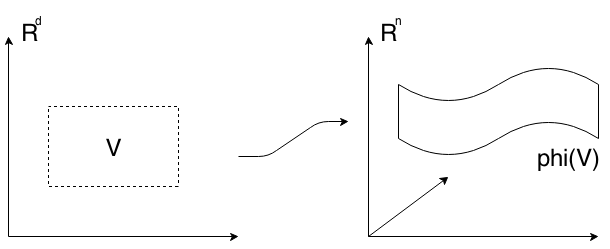
\includegraphics[scale=0.5]{pictures/MA2_0001}
\begin{beispiel}[reguläre Kurven $\varphi:I\subset\mathbb{R}\rightarrow\mathbb{R}^n$]
Dabei ist $I$ offen und der Tagentialvektor nirgendwo identisch mit dem Nullvektor, also $\varphi'(x)\neq 0$
\begin{enumerate}
\item $\varphi:(0,2\pi)\rightarrow\mathbb{R}^2$ mit $\varphi(t)=\begin{pmatrix}
\cos kt \\ \sin kt
\end{pmatrix}$ und $k\in\mathbb{N}_{\geq 2}$\\
\begin{center}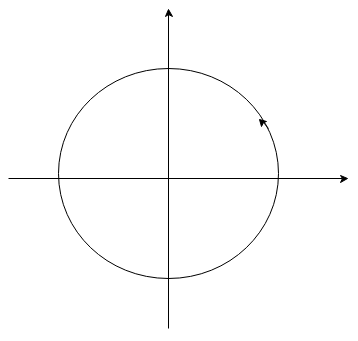
\includegraphics[scale=0.3]{pictures/MA2_0002}\\ \end{center}
Der Einheitskreis wird hier k-mal durchlaufen. Da $\varphi'(x)\neq 0$, ist $\varphi$ regulär.
\item $\varphi(-\pi,\pi)\rightarrow\mathbb{R}^2$ mit $\varphi(t)=(1+2\cos t)\begin{pmatrix}
\cos t \\ \sin t
\end{pmatrix}$\\
\begin{center}
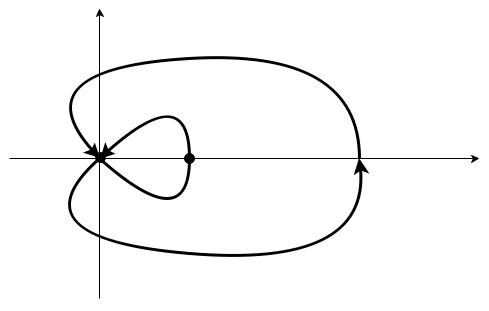
\includegraphics[scale=0.3]{pictures/MA2_0003}\\
\end{center}
$\varphi(\pm\frac{2\pi}{3})=\begin{pmatrix}
0 \\ 0
\end{pmatrix}, \ \varphi(0)=\begin{pmatrix}
3 \\ 0
\end{pmatrix}$\\
$\begin{pmatrix}
1 \\ 0
\end{pmatrix}$ \ gehört \textbf{nicht} zur Kurve ("$=\varphi(\pm\pi)$") und $\varphi$ ist regulär.
\item $\varphi:(-1,1)\rightarrow\mathbb{R}^2$ \ mit \ $\varphi(t)=\begin{pmatrix}
t^3 \\ t^2
\end{pmatrix}$ \ ist wegen $\varphi'(0)=0$ \ \textbf{nicht} regulär\\
\begin{center}
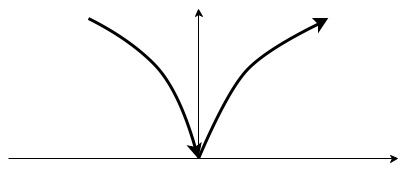
\includegraphics[scale=0.3]{pictures/MA2_0004}
\end{center}
\end{enumerate}
\end{beispiel}
\ \linebreak
\begin{beispiel}[Parametrisierung von Graphen]
Sei $f\in C^q(V,\mathbb{R}^{n-d})$,\\
$V\subset\mathbb{R}^d$. Betrachtet wird $\varphi:V\rightarrow\mathbb{R}^n$ mit $\varphi(x)=(x,f(x))$\\
\begin{center}
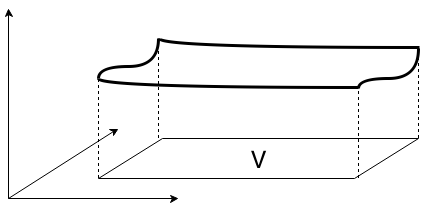
\includegraphics[scale=0.5]{pictures/MA2_0005}\\
\end{center}
$\varphi$ ist regulär, da offenbar $\varphi\in C^q(V,\mathbb{R}^n)$ und $\varphi'=\begin{pmatrix}
id^d \\ f'(x)
\end{pmatrix}\in\mathbb{R}^{n\times d}$ \ ist.\\
\linebreak
\end{beispiel}
Es folgt eine Wiederholung zur \textbf{Relativtopologie} (vgl. Kapitel 14). Wir wissen, dass $U\subset M$ genau dann offen bezüglich $M$ ist, wenn es ein $\tilde{U}\subset\mathbb{R}^n$ gibt, dass offen ist, und das $U=\tilde{U}\cap M$ erfüllt. Später wird $M$ eine Mannigfaltigkeit sein und wir werden untersuchen, was in ihr offen ist.\\
\begin{center}
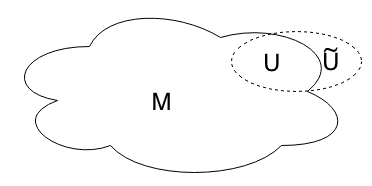
\includegraphics[scale=0.5]{pictures/MA2_0006}\\
\end{center}
Auf dieser Grundlage lässt sich auch der Begriff der \textbf{Umgebung} definieren:\\
$U\subset M$ heißt nämlich genau dann Umgebung von $u\in M$ bezüglich $M$, wenn es ein bezüglich $M$ offenes $U_0\subset M$ gibt, in dem $u$ liegt und das Teilmenge von $U$ ist.\linebreak\linebreak
\newpage
\textbf{\textsf{Beispiel für}} \ $M\subset\mathbb{R}^n$.\\

\begin{center}
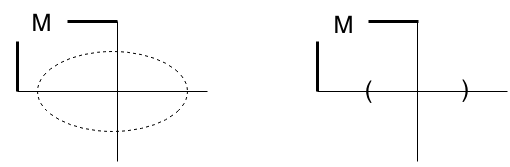
\includegraphics[scale=0.5]{pictures/MA2_0007}\\
\end{center}
\hspace{70pt} offen bzgl. M \hspace{70pt} nicht offen bzgl. M\\

\begin{definition}[Mannigfaltigkeiten]
Wir nennen $M\subset\mathbb{R}^n$ eine \textbf{d-dimensionale $C^q$-Mannigfaltigkeit} ($q\in\mathbb{N}_{\geq 1}$), falls

\begin{enumerate}
\item es für alle $u\in M$ eine (offene) Umgebung $U$ von $u$ bezüglich $M$ gibt und
\item es eine reguläre $C^q$-Parametrisierung $\varphi:V\subset\mathbb{R}^d\rightarrow\mathbb{R}^n$ ($V$ ist offen) existiert, die homöomorph ist und in die Mannigfaltigkeit abbildet (also \  $\varphi(V)=U$).
\end{enumerate}
\emph{Wiederholung: Eine stetige Abbildung heißt homöomorph, falls eine Umkehrabbildung existiert, die auch stetig ist.}\\
\end{definition}
In der Literatur wird $M$ auch manchmal als $C^q$-\emph{Unter}mannigfaltigkeit bezeichnet. Wir werden jedoch später zeigen, dass die verschiedenen Definitionen von Mannigfaltigkeiten gleichwertig sind.\\
Da ab jetzt immer hauptsächlich $C^1$-Mannigfaltigkeiten auftauchen werden, werden wir diese in Zukunft einfach "Mannigfaltigkeiten" nennen.\\

\begin{center}
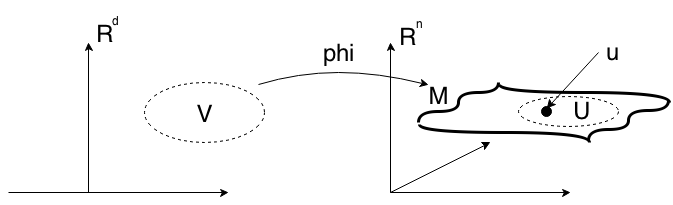
\includegraphics[scale=0.5]{pictures/MA2_0008}\\
\end{center}
Die Umkehrabbildung $\varphi^{-1}$ beziehungsweise ($\varphi^{-1}, U$) nennt man die \textbf{Karte} von $M$ um $u\in M$, wobei $U$ das zugehörige \textbf{Kartengebiet}, $\varphi$ selbst die Parametrisierung und $V$ der Parameterbereich ist.\\
Karten können eine Mannigfaltigkeit jedoch nur lokal beschreiben. Aus diesem Grund führt man den Begriff des Atlas, der eine globale Beschreibung ermöglicht, ein:\\
Die Menge $\{\varphi^{-1}_\alpha | \alpha\in A\}$ heißt \textbf{Atlas} der Mannigfaltigkeit M, falls die zugehörigen Kartengebiete $U_\alpha$ jene vollständig überdecken.\\
\linebreak
Weiterhin wichtig ist der Begriff der sogenannten \textbf{Einbettung}, bei der es sich um eine reguläre Parametrisierung handelt, die homöomorph ist. Wir vereinbaren, dass es sich im folgenden bei allen Parametrisierungen von Mannigfaltigkeiten stets um Einbettungen handelt.
\begin{beispiel}[Beweise bitte Selbstudium]\ \\

\begin{enumerate}
\item Der Kreis aus Beispiel 1.1 ist eine 1-dimensionale $C^\infty$-Mannigfaltigkeit, obwohl der Kreis k-fach durchlaufen wird. Der Atlas benötigt mindestens zwei Karten.
\item Die Kurven aus Biespiel 1.2 und 1.3 sind keine Mannigfaltigkeiten, da $\varphi$ nicht überall homöomorph ist.
\item Jedes offene $M\subset\mathbb{R}^n$ ist eine n-dimensionale $C^\infty$-Mannigfaltigkeit mit $\{id\}$ als Atlas.
\end{enumerate}
\end{beispiel}

\begin{beispiel} Sei $M:=\graph f$ aus Beispiel 2. Offenbar ist 
$\varphi:V\subset\mathbb{R}^d\rightarrow M\subset\mathbb{R}^n$ 
eine Einbettung. Das macht $M$ zu einer d-dimensionalen $C^q$-Mannigfaltigkeit.
\end{beispiel}

\begin{beispiel}
Sei $f:D\subset\mathbb{R}^n\rightarrow\mathbb{R}^{n-d}$ ($D$ offen) q-fach stetig differenzierbar für $q\geq 1$. Offenbar ist

\begin{equation}
\rang f'(u)=n-d \ \ \ \ \ \ \ \forall u\in D
\end{equation}
Wir nennen $M=\{u\in D \ | \ f(n)=0\}$ die Niveaumenge von $f$\\

\begin{center}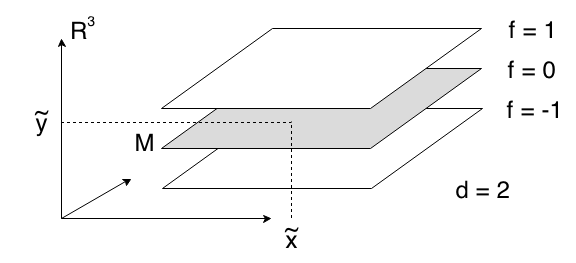
\includegraphics[scale=0.5]{pictures/MA2_0009}\\
\end{center}
Fixieren wir $\tilde{u}=(\tilde{x},\tilde{y})=(x_1,...,x_d,y_1,...,y_{n-d})\in M$
, so sehen wir mit (29.3) und eventuellen Koordinatenvertauschungen, dass 
$f(\tilde{x},\tilde{y})$ regulär ist. Der \emph{Satz über implizite Funktionen}
sichert uns nun, dass es eine Umgebung $V\subset\mathbb{R}^d$ von $\tilde{x}$, 
eine Umgebung $W\subset\mathbb{R}^{n-d}$ von $\tilde{y}$ und ein 
$\psi:V\rightarrow W\in C^q(V,W)$ gibt, das $(x,\psi(x))\in M$ erfüllt und homöomorph ist.\\
Es folgt, dass $\varphi:V\subset\mathbb{R}^d\rightarrow\mathbb{R}^n$ mit 
$\varphi(x)=(x,\psi(x))$ eine homöomorphe, reguläre Einbettung  und $\varphi(V)$ 
Umgebung von $\tilde{u}\in M$ bezüglich von $M$ ist. Daraus können wir nun schließen, 
dass $M$ eine d-dimensionale $C^q$-Mannigfaltigkeit ist.\\
\linebreak
\emph{Bemerkung: $M=\graph f$ und $M=\{f=0\}$ sind grundlegende Konstruktionen 
für Mannigfaltigkeiten. \textbf{Lokal} ist jede Mannigfaltigkeit von dieser Gestalt!}
\end{beispiel}
\end{document}
